% Use only LaTeX2e, calling the article.cls class and 12-point type.

\documentclass[10pt,oneside]{article}
\def\thesisversion{net}
% Users of the {thebibliography} environment or BibTeX should use the
% scicite.sty package, downloadable from *Science* at
% www.sciencemag.org/about/authors/prep/TeX_help/ .
% This package should properly format in-text
% reference calls and reference-list numbers.
\usepackage{LukeThesis}
\usepackage[utf8]{inputenc} 
\usepackage{calc}
\usepackage{float}
\usepackage{titlesec}  

\usepackage{changepage}   % for the adjustwidth environment

% Use times if you have the font installed; otherwise, comment out the
% following line.
\usepackage{times}

\titleformat{\section}{\Large\bfseries}{\thesection}{0.5em}{}
\titleformat{\paragraph}{\small\bfseries}{\theparagraph}{0.5em}{}

\titlespacing\section{0pt}{4pt}{0pt} %[MARIUS]:change the middle value if you want to change the spacing of the section
\titlespacing\subsection{0pt}{2pt}{0pt}%[MARIUS]:change the middle value if you want to change the spacing of the subsection
\titlespacing\subsubsection{0pt}{1pt}{0pt}%[MARIUS]:change the middle value if you want to change the spacing of the subsubsection
\titlespacing\paragraph{0pt}{1pt}{0pt}%[MARIUS]:change the middle value if you want to change the spacing of the paragraph

\setlength\parindent{0pt} % sets indent to zero
\setlength{\parskip}{7pt} % changes vertical space between paragraphs




% writtenby skal måske layoutes lidt anderledes
%\newcommand{\writtenby}[1]{\vspace*{-18pt}\hfill#1\vspace{18pt}\newline}
% \newcommand{\writtenby}[1]{\vspace*{-36pt}\hfill#1\vspace{12pt}\newline}


\newcommand{\fig}[1]{Figure~\ref{fig:#1}}
\newcommand{\tbl}[1]{Table~\ref{tbl:#1}}
\newcommand{\glos}[1]{(Glossary: ~\ref{glos:#1})}
\newcommand\writer[1]{\nobreak\begin{flushright} \vspace{-0.6cm}\small\textbf{Author: \textit{#1}}\end{flushright} \vspace{-0.5cm}}

\renewcommand{\b}[1]{\textbf{#1}}
\renewcommand{\i}[1]{\textit{#1}}

%
%==================================================================================================
% SECTION NUMBERING SETUP
%==================================================================================================
\setcounter{tocdepth}{2}                            %2 adds sections up to subsections
\setcounter{secnumdepth}{5}                         %Subsubsections get a number when this is
%\setcounter{section}{1}

% The preamble here sets up a lot of new/revised commands and
% environments.  It's annoying, but please do *not* try to strip these
% out into a separate .sty file (which could lead to the loss of some
% information when we convert the file to other formats).  Instead, keep
% them in the preamble of your main LaTeX source file.


% The following parameters seem to provide a reasonable page setup.

%\topmargin 0.0cm
%\oddsidemargin 0.2cm
%\textwidth 16cm 
%\textheight 21cm
%\footskip 1.0cm


%The next command sets up an environment for the abstract to your paper.

%\newenvironment{sciabstract}{%
%\begin{quote} \bf}
%{\end{quote}}


% If your reference list includes text notes as well as references,
% include the following line; otherwise, comment it out.

%\renewcommand\refname{References and Notes}
\begin{document} 
%==================================================================================================
% FRONT PAGE
%==================================================================================================
\begin{titlepage}
\begin{center}

\includegraphics[width=0.15\textwidth]{figures/DTU-logo.pdf}\\[1.3cm]

\textsc{\LARGE Technical University of Denmark}\\[0.8cm]
\textsc{\LARGE Artificial Intelligence \\[0.1cm]and Multi-Agent Systems}

% Title
{
 \vspace{1.5cm}
 \huge \bfseries Final Project Report}\\
 \vspace{2.5cm}
 \rule{\linewidth}{0.1mm} \\[0.4cm]
%\hrule \\[1.5cm]
% Author and supervisor
\begin{minipage}{0.4\textwidth}
    \begin{flushleft} \large
	\emph{Authors:}\\
    Albert Fernández de la Peña \\
    Cosmin Stefan Dobrin\\
    Javier Calvo\\
    Marius Constantinescu\\
    Rafaela-Ioana Voiculescu\\
	Ruxandra Nistor
	\end{flushleft}
\end{minipage}
\begin{minipage}{0.4\textwidth}
	\begin{flushright} \large
	\emph{Student numbers:} \\
    s112213\\
    s121038\\
    s110747\\
    s121039\\
	s120931\\
    s121037
	\end{flushright}
\end{minipage}
\vfill
% Bottom of the page
{\large \today}
\end{center}

GROUP: BlueDucks

\footnotesize ** This document was written together by all the members of the team. The main writers for each
of the sections have been indicated, however \textbf{all members have contributed} to the general structure
and to the revising of the content. Regarding the implementation, each of us had \textbf{equal contributions}
and, in a project of this size, it is hard to mention the exact parts of code on which each team member worked
on.
\end{titlepage}



%%%%%%%%%%%%%%%%% END OF PREAMBLE %%%%%%%%%%%%%%%%




% In setting up this template for *Science* papers, we've used both
% the \section* command and the \paragraph* command for topical
% divisions.  Which you use will of course depend on the type of paper
% you're writing.  Review Articles tend to have displayed headings, for
% which \section* is more appropriate; Research Articles, when they have
% formal topical divisions at all, tend to signal them with bold text
% that runs into the paragraph, for which \paragraph* is the right
% choice.  Either way, use the asterisk (*) modifier, as shown, to
% suppress numbering.

\section{Introduction}


%if someone feels more inspired, please change this%

This report aims to present an approach to a multi-agent system. The goal was to create a multi-agent system in which agents had to transport boxes on goal cells by pushing or pulling them. This report analyses the problem and presents our solution, focusing on our results and findings.

We have implemented a multi-agent system for a problem-specific domain, which uses hierarchical planning and forward state search. The result is satisfactory, with the system behaving well in most of the maps that were used for testing. However, with more work in the heuristics part, even better results could be achieved.
%still need to "Tease" a bit about the findings. Maybe after we've written them..%


\section{Problem analysis}
\label{sec:problem}
\writer{Rafaela, Ruxandra}
The first step when starting to work on the project was to decide upon the general architecture of our
implementation. When dealing with a system of this amplitude it is best to start testing individual components
as soon as possible. Module testing ensures that everything that needs to be integrated, has been previously
tested and verified.

Besides ensuring the modularity of the system, a decision that has to be made from the beginning is whether to
use \textbf{multibody planning} or \textbf{multi-agent planning}. While both have their advantages, each of
them is applicable in different scenarios. Multibody planning is preferred when dealing with an environment
where state exploration is very efficient due to low branching factor. However, when planning on a large scale
with many possible alternative actions, where the branching factor is very large, a solution based on
multi-agent systems reacts better.

The next step was analysing to which extent the environment, the number of agents and the unpredictable
obstacles affect the performance and the decision making process. Before starting to compute the plan for
achieving the goals, a \textbf{pre-analysis} of the existent paths, patterns and goal, as well as the
complexity of the environment must be made.

Even though a good knowledge of the map is useful, the way the states are explored can dramatically affect the
performance. When doing blind state exploration the branching factor can exponentially escalate. To create a
good heuristic, the data from the pre-analysis should be used, though a comprehensive analysis of the  current
state is essential. However, considering the high branching factor, a complete analysis of the current state
would take an unacceptable amount of time. Aside from time, memory resources need to be kept in mind when
dealing with high branching factors, as very large number of states are being generated. Thus, a
\textbf{compromise} between having the optimal solution and finding the least computationally expensive
solution needs to be found. Compromises include using \textbf{heuristics} and \textbf{pruning} of states
during the exploration.

The problems analysed up to this point regard mostly single agent systems. In the case of multi-agent systems,
such as the one we are dealing with, other problems should be considered. Even when dealing with only two
agents, cases where the agents have conflicting plans might occur. In some cases, the \textbf{conflict}
appears just because the agents have not chosen their goals in the proper order. This can easily be solved by
\textbf{reordering/ replanning} of goals. In other cases, in order to avoid conflicts, the plans of the agents
could be merged by \textbf{postponing actions}. This is not always possible as two agents might need to access
common resources. Furthermore, for very big plans or for a large number of agents, the number of possibilities
to interlace the agents’ plans is very big and, as such, it could lead to wasting a lot of time and resources
on computing the solution. When plan merging is not an option, other approaches can be taken. Among them,
there are the \textbf{inter-agent communication} and the \textbf{high-level conflict solving}.

The communication between agents can also prove to be problematic as it can introduce synchronization problems
which can lead to cases like multiple agents being assigned the same goal or a goal not being assigned to any
agent. For this problem, solutions that involve direct interagent communication like
FIPA-ACL\footnote{FIPA-ACL \url{http://www.fipa.org/repository/aclspecs.html}}  can be used, as well as
solutions that involve communication being performed through a central entity.

When conflicts arise, there is the option to make agents communicate in order to solve the conflict and decide
upon a plan or the option for the agents to resort to a central entity that tells them what to do in order to
solve the conflict. In some cases, a hybrid solution between the two can also be used.

For the case where unknown objects are present in the environment, special approaches need to be taken into
consideration. As replanning could be triggered at any moment due to detection of unknown objects, it is not
that important to have a complete and optimal plan, but to be able to compute an acceptable plan in a short
amount of time. Also, when dealing with multiple agents, not all agents need to recompute the plan when
another agent identifies an unknown object.

As it is expected, the number of things that need to be taken into consideration for elaborating efficient and
optimal solutions is very large and a compromise should always be found between all the factors involved, as
some will prove to be more important in some cases while others in other cases.




\section{Solution}
\label{sec:solution}
\subsection{Approach}
\writer{Albert}

\label{sec:approach}

This section presents our approach to the project. We have implemented a \textbf{multi-agent} infrastructure
based on a Beliefs - Desires - Intentions model. The defined domain is \textbf{problem specific} and thus
several environment specific \textbf{pre-analyses} are done to reduce the complexity of the problem during
running. Complex goals are handled by decomposing them in simpler ones using \textbf{hierarchical planning}.
For each task, a plan is then computed using \textbf{forward state search}. Moreover, \textbf{specific
heuristics} have been developed for each of the tasks. The system is multi-agent and each of the agents plans
for its own goals and cooperates with the others. In order to solve conflicts, \textbf{merging of plans} by a
central entity has been implemented, although for cases where it is not feasible, \textbf{conflict-solving}
replanning together with \textbf{inter-agent communication} is then used. Details regarding each of these
aspects are presented in the following sections.

Our system implementation has been developed in Java. Due to the nature of the project, where processing time
has to be radically reduced due to the size of the level maps, throughout the implementation we have used a
multitude of data structures and low-level optimization. This has made the state expansions, heuristic
computations and all the required processing as fast as possible.

\subsection{Architecture}
\label{sec:architecture}
\writer{Cosmin}

% Architecture subsection content

As mentioned in subsection~\ref{sec:approach}, we are using a multi-agent infrastructure, with a central
entity that handles the communication between agents and all the synchronisation issues. A diagram showing the
most important components in our implementation can be seen in Figure~\ref{fig:architecture}.

\begin{figure}[htb]
\begin{center}
 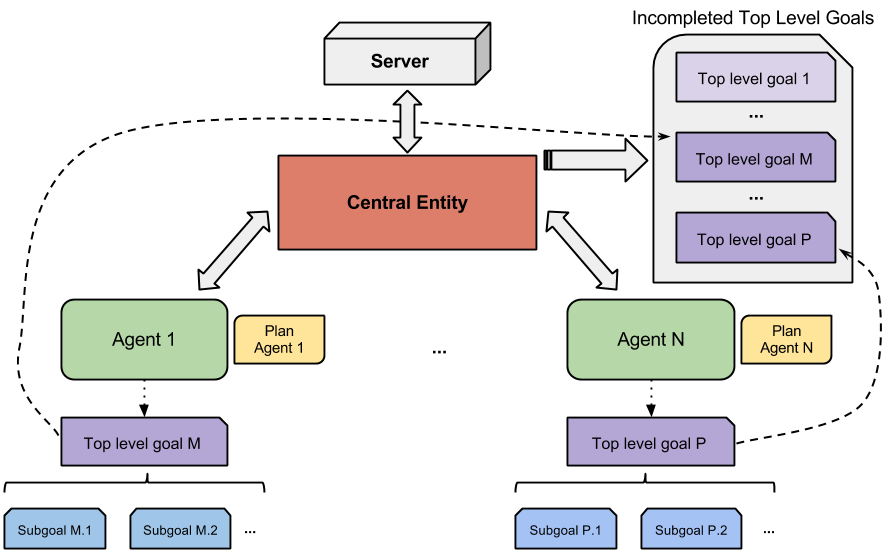
\includegraphics[width=0.92\textwidth]{figures/architecture.png}
 \caption{General system architecture}
 \label{fig:architecture}
\end{center}
\end{figure}

As it can be observed from the figure, the system's main components are a central entity and a set of agents.
The central entity maintains a set of top level goals that need to be completed for a level to be solved. Each
of the agents gets assigned one of these goals and is responsible for breaking it into smaller and easier
subgoals and for elaborating a plan to complete them.

The central component of our application is depicted as the \textbf{Central Entity}. Among the tasks that are
handled by it we can enumerate:

\vspace{-12pt}
\begin{itemize}
\setlength{\itemsep}{0cm}
\item coordinate the communication between the agents
\item manage the list of top level goals that need to be completed (Desires)
\item decide which agents work on which goals (in situations when multiple agents have proposals for the same goal)
\item merge agents' plans, if possible
\item coordinate the communication between agents when plan merging conflicts appear
\item handle communication with the server
\item maintain a real, up-to-date representation of how the level map looks like (Beliefs)
\end{itemize}
\vspace{-0.3cm}

Each of the agents in the system handles the following tasks:

\vspace{-12pt}
\begin{itemize}
\setlength{\itemsep}{0cm}
\item make proposals for each of the goals it can handle
\item divide the goals into easier subgoals
\item make a plan for completing its goal
\item make a plan to solve a plan merging conflict, if requested
\item make a plan to help other agents with clearing paths, if requested
\end{itemize}

\vspace{-0.3cm}
\begin{figure}[!htb]
\begin{center}
 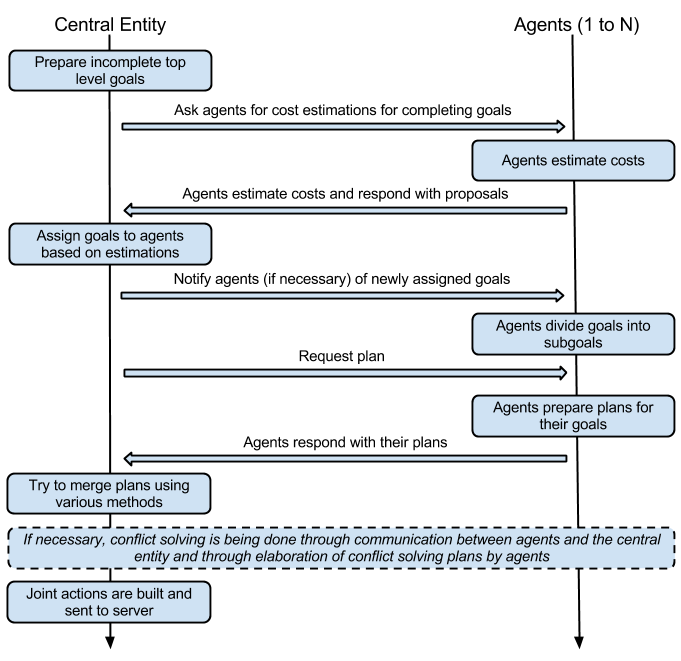
\includegraphics[width=0.75\textwidth]{figures/communication_flow.png}
 \caption{Brief representation of important steps and communication flow}
 \label{fig:communication_flow}
\end{center}
\end{figure}

Figure~\ref{fig:communication_flow} shows the most important steps followed by our implementation and the
communication flow between the agents and the central entity. The diagram only depicts a full iteration of the
steps and it has to be mentioned that, while running, some of the steps and communication messages shown might
not be applicable or are skipped for optimization reasons. More details about these situations will be
provided in the following subsections.

Initially, the central entity is identifying the top level goals that still need to be completed.
Subsequently, agents are asked to compute an estimation of the cost of the plan for solving those goals (if
applicable). Based on these estimations, the central entity then assigns goals to the agents. After this step,
agents break down the goals into subgoals that are easier to use and for which different heuristics can be
applied. Then an AStar-based search is used to identify a plan. These plans are then collected by the central
entity, which tries to merge them using various methods. If the merge is successful, the joint actions are
extracted and sent to the server for each turn. If the plans for some of the agents cannot be merged, the plan
merging conflicts are solved under the coordination of the central entity. All these steps and the actual
implementation are presented with more details in the following subsections.


\subsection{Techniques}

\subsubsection{Preanalysis}
\writer{Albert}
As identified in Section~\ref{sec:problem}, an early analysis of the map could provide valuable information to
be used by the agents when exploring states. For example, using the Dijkstra distance instead of Manhattan
improves the correct choice of goals. Therefore, after initializing the map, the following analyses were
precomputed for further use by the agents. The first step consisted in creating an initial graph, where
vertices are the cells and the edges represent the links to their respective neighbours.

\paragraph{Dijkstra distance}

In order to provide the agents with the most accurate approximation of the real distance between two cells, we
considered that the best approach was to use \textit{Dijkstra's algorithm}, which is a graph search algorithm
that computes the shortest path distance between a cell (vertex) and every other cell.

With this solution, we were able to make the agents go for the closest \textit{accessible} goal. When using
the Manhattan distance, the agents go for a goal which is falsely considered to be closer, although there are
walls in between and the real distance is larger.

We have found, however, that for certain maps which exceed a certain dimension, the analyses is
computationally very expensive and the time consumed by the computation of Dijkstra's graph is too large or
contains too many free cells. For these maps, in order to be able to complete them within the maximum time of
the competition, we decided that we would use Manhattan distance instead.

\paragraph{Betweenness Centrality}

The problem analysis also states that identifying the relevant cells in a map is important in order to avoid
blocking them or in order to allow the agents know which goal cells have to be completed first. Therefore,
with the network graph that we had previously built, we could use a measure such as the betweenness centrality
of a node. This measure consists of the number of shortest paths from each vertex to all others, that pass
through the evaluated node. In Figure~\ref{fig:hanoi} we present an example of the betweenness centrality
measure for the cells of \textit{Boxes of Hanoi} map. It can be observed that cells situated at the end of
each column had a score of 0, while the top row had the higher scores. Thus, this property can be used in
heuristics for penalising agents that leave boxes in important cells or for determining important goals.

\begin{figure}[htb]
\begin{center}
 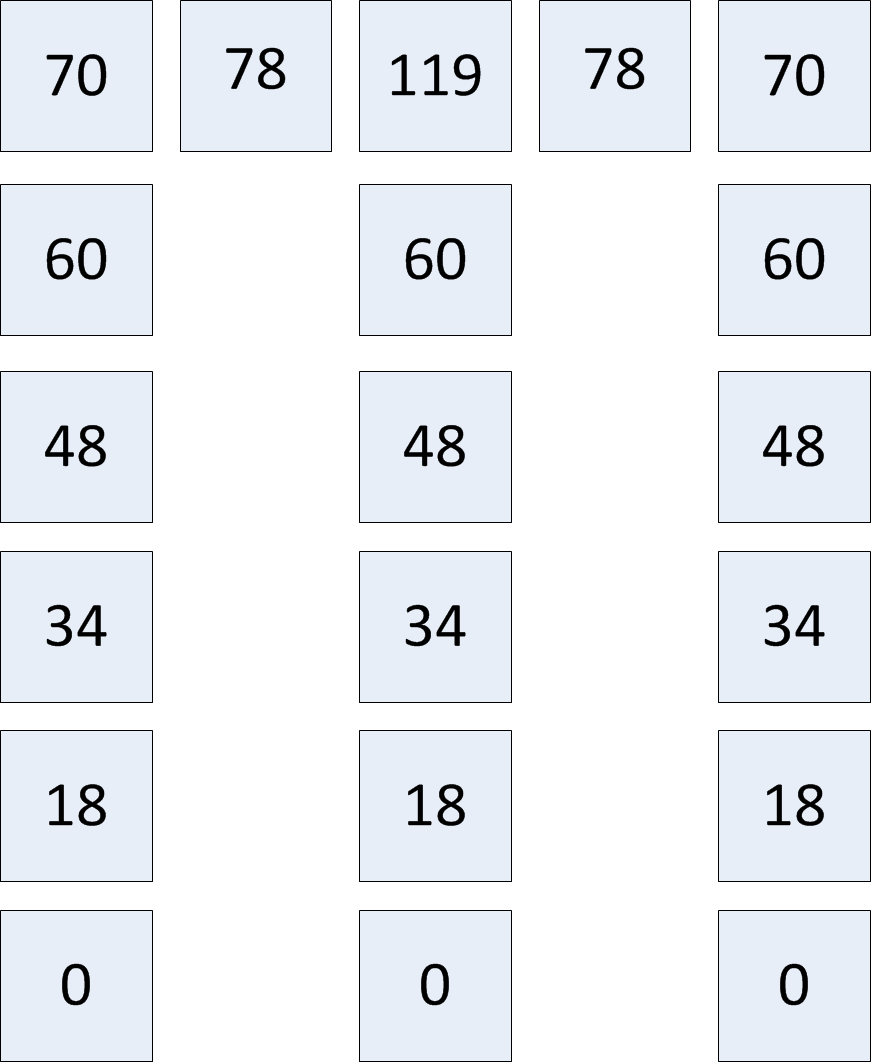
\includegraphics[width=0.3\textwidth]{figures/hanoi.png}
 \caption{Betweenness centrality for the Boxes of Hanoi map}
 \label{fig:hanoi}
\end{center}
\end{figure}

Once again, this is an expensive metric, having a cost of $O(|V|^2log|V| + |V||E|)$. Therefore, for those maps
for which the cost was too large, and thus would make the system not be able to finish on time during the
competition, this property was not computed and a default value was given to all the cells.

\paragraph{Degree Centrality}

Another property that can be easily obtained after building the network graph is the degree centrality, which
is the number of links that a node has\footnote{In our case, the number of neighbours of each cell}. This
measure is useful to identify those cells that, even though they have a high betweenness centrality, also have
many neighbours (4), and thus, should not have as much importance as the ones that could block a path.

\paragraph{Group of goals}

The last analysis that is precomputed is the identification of groups of goals, as for example in
Figure~\ref{fig:goalshanoi}. Being able to recognize groups of goals was defined as crucial, especially in
cases of maps similar to boxes of Hanoi. Therefore, we built an algorithm that for each goal analyzed if there
is any neighbour goal, and recursively, computes the whole group. The usage of these groups permits the agent
to complete first the cells that are part of a group and that have a lower betweenness centrality, meaning the
ones that do not block other goals.

\begin{figure}[htb]
\begin{center}
 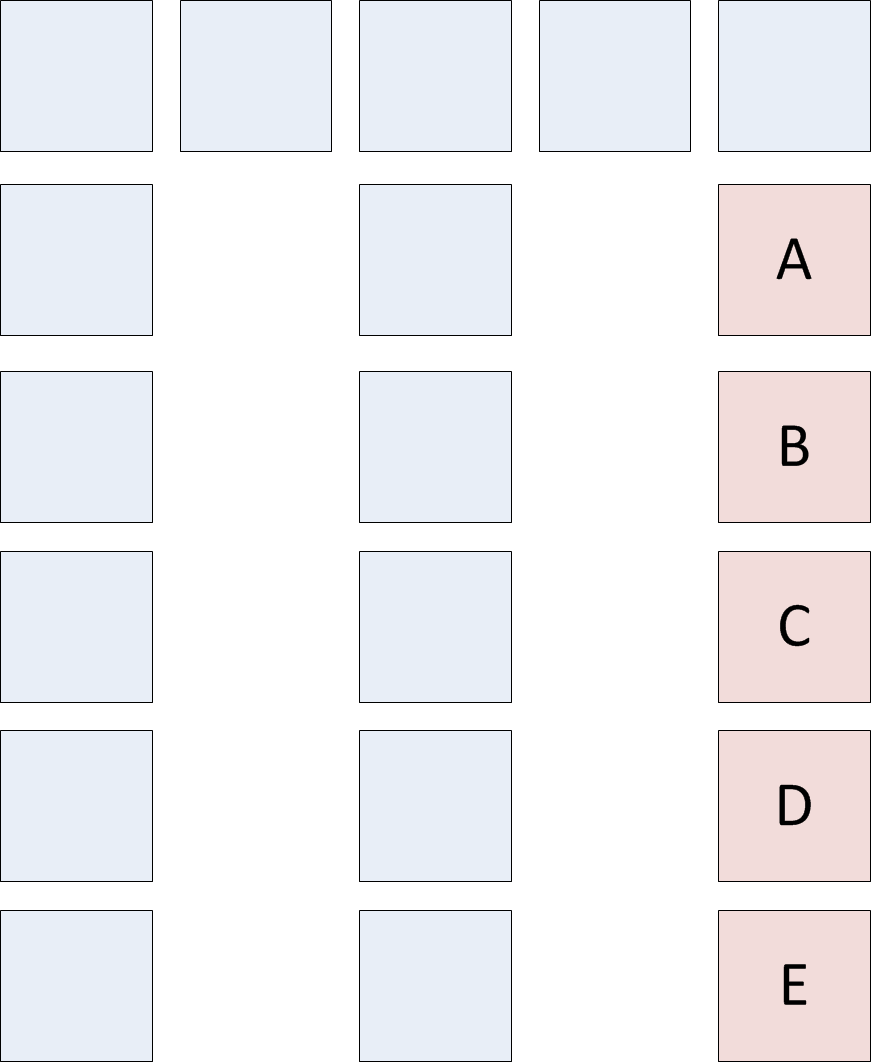
\includegraphics[width=0.3\textwidth]{figures/goalshanoi.png}
 \caption{Identification of groups of goals cells}
 \label{fig:goalshanoi}
\end{center}
\end{figure}


\subsubsection{Goal picking}
\writer{Albert}
As stated, one of the major challenges was to properly select the goals correctly, especially the order in
which they were going to be completed; choosing an incorrect order could lead to an unresolvable state.

In our architecture, the Central Entity is responsible for computing all the top level goals needed to be
completed by the agents and for asking the agents for an estimation of the cost that would require them to
complete each goal.

For computing this cost, specific heuristics for each top level goal were designed. For instance, for the
\textit{DeliverBoxGoal}\footnote{The top level goal saying that a particular box has to be delivered to a
particular cell}, the following properties were taken into account, with different importance:


\vspace{-12pt}
\begin{enumerate}
\setlength{\itemsep}{0cm}
    \item Distance (Dijkstra/Manhattan) between the agent, the box, and the goal.
    \item Betweenness centrality of the cell in which the box was.
    \item Distance from the goal cell to other boxes.
    \item Betweenness centrality of the goal cell.
    \item Blocking another goal by solving this one.
    \item Undoing a goal.
\end{enumerate}
\vspace{-0.3cm}

Choosing the correct value is a complex issue: giving too much importance to one of the properties would mean
that others might not even be able to influence the final score. There are two of them that are penalized with
a high value: blocking other goals and undoing goals. Also, goals situated in cells with lower betweenness
centrality are considered to be better alternatives if possible to use, so it was important to penalize the
rest.

% SHOULD WE ADD THE FORMULA??

\subsubsection{Exploration}
\writer{Rafaela}
State exploration is necessary in order to determine the best possible alternative an agent has for achieving
its goal. Our project tackles the exploration problem by using the A-Star approach together with various types
of heuristics which depend on the types of goals, the results of the pre-analysis of the map, etc. (the
heuristics are described in Section \ref{sec:heuristics}). This approach enables the finding of the path
closest to the optimal solution.

\subsubsection{State}
\writer{Ruxandra}
As the A-Star algorithm used to explore the states for each agent can expand a very high number of states, we
need to take care what we include in a state. A state is defined by the configuration of boxes on the map as
well as the agent for which the state is calculated. We chose to ignore the other agents when doing state
expansion, as taking them into account would not be useful for our purpose. Everything else related to the map
was kept in a separate, common resource.

Even though we try to keep as little information as possible in a state, for large maps with high number of
boxes, we still encountered memory problems. To solve this, we kept all the references to the boxes in the
common resource and used only indexes to cells and boxes in the actual state. Furthermore, to know which cells
are occupied we used a BitSet to save space and speed up computations.

However, in the expansion we noticed that, in some situations, the algorithm was expanding slower than it
should have. After doing some testing we have realized that for a high number of states, the collisions
between the hash-codes\footnote{Used in various types of data structures} of the states would be very high.
This is why we implemented our own hashing method for the states. For optimality reasons, when creating a new
state based on a previous state, we used the hash of the previous state to which we add/ subtract values
depending on the differences between the two states (boxes' positions/ agent's position). This optimization
helped in expanding the states faster as it is easier to compute the hash, but also because the hash is better
suited for the problem and gives fewer conflicts.

\newpage % to make it look good on a new page
\subsubsection{Plan merging}
\writer{Rafaela}
\label{sec:plan_merging}

In multi-agent systems, as mentioned in the section \ref{sec:architecture}, one of the most important aspects
to be considered is how plans originating from multiple agents are merged together, so that no actions are
conflicting and that no resources are used at the same time.

Our approach to plan merging is to find whether there is an optimal way to intercalate the agents’ actions in
order to avoid illegal situations\footnote{For example, when 2 agents try to move in the same cell or push the
same box}, possibly delaying the actions of some of the agents. Our aim is to offer an optimal plan merging
solution, in case such a plan merging is possible. A plan merging fails when, no matter the number of NoOp
actions that one or multiple agents perform, a solution for all of them to achieve their respective goals is
impossible.

Two alternatives were considered for merging multiple plans. The first one was to merge all the agents' plans
into one plan at once. The second solution was to merge the plans one at a time: the first plan with the
second one, then the result with the third one and so on. After analysis, we have agreed that the best option
for us is to try to merge the plans of all active agents (agents that have goals) at the same time. This
decision is supported by the fact that, in this way, it is easier to identify which agents’ plans collide. In
the second option of merging the problem is that identifying which agents have conflicting actions is almost
impossible after we have already computed a merged plan for other agents.

For trying out all possible solutions of merging the agents’ plans, we are using an algorithm based on
backtracking, that loops through all options of intercalating agents’ possible actions. At each step, it tries
to fit as many possible actions from the agents’ plans and delay the other actions. Furthermore, the states
that result after applying a set of actions are only computed (expanded) when and if is necessary, for
optimisation reasons.  An example for how the algorithm works for three agents is shown in Figure
\ref{fig:plan_merging} \footnote{The red colored option is generated but cannot be used due to incompatible
actions, the green option is valid so can be expanded while the grey nodes are not even generated or expanded.
The dash displayed in some nodes represents that a NoOp action has been introduced for the respective agent.}.

\begin{figure}[htb]
\begin{center}
 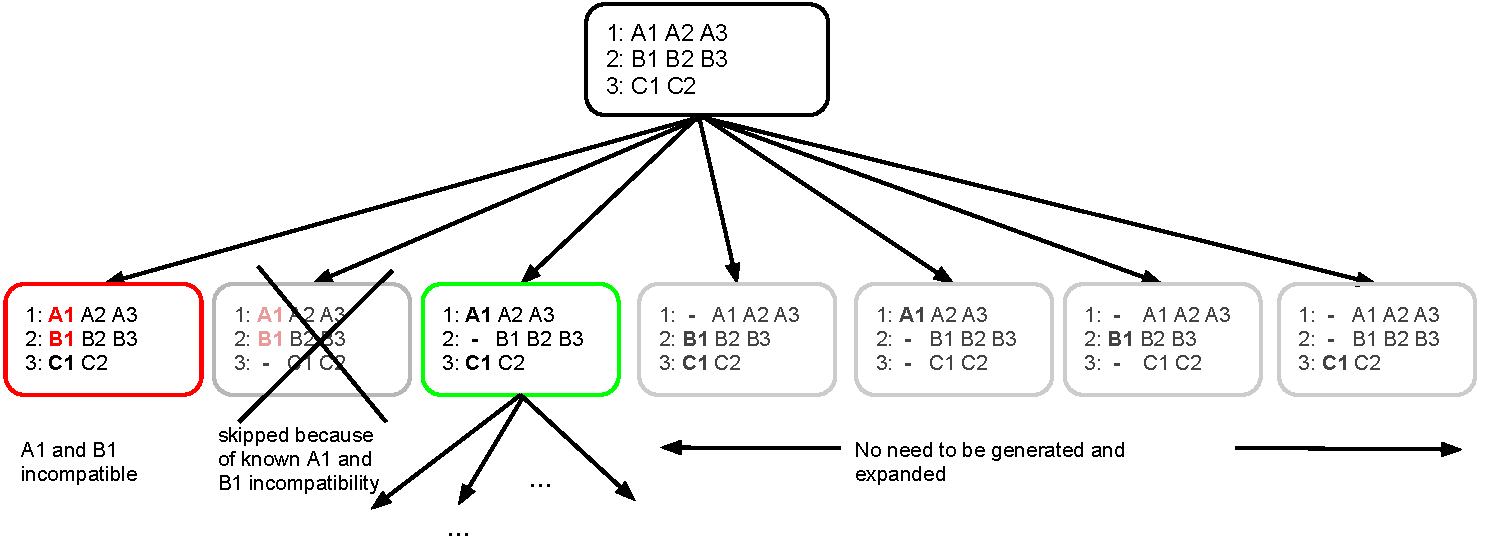
\includegraphics[width=\textwidth]{figures/plan_merging.pdf}
 \caption{Tree for merging}
 \label{fig:plan_merging}
\end{center}
\end{figure}

As it can be seen in Figure \ref{fig:plan_merging}, when we try to merge plans for all three agents, we have
an incompatibility between actions from agents 1 and 2 (actions A1 and B1). The backtracking algorithm will go
back and try other options. For optimisation reasons, our algorithm does not even try to expand the second
option (having active agents 1 and 2 and give agent 3 a NoOp action), because we already know from the
previous try that agents 1 and 2 cannot be active at the same time at this point. The algorithm moves to the
following option and tries to keep the actions from agents 1 and 3 while agent 2 has a NoOp action. This, for
the assumed case, works and the backtracking algorithm will move forward to analyse the next actions remaining
for all agents in a similar way. Assuming that the algorithm will find a solution on this branch, all the
following possibilities from this level (activating agents 2 and 3, or just agent 1, or just agent 2 or just
agent 3) are not even generated (not to mention expanded). This approach saves a lot of resources of time and
memory.

Another optimisation we brought to this algorithm is that we pre-generate lists with all possible options of
activation for agents. The lists contain true or false depending if the agents can perform their action or
have a NoOp action at a certain level. Since we pre-generate and save these options, there is no need to
generate them each time we move to a new level in the options’ graph with the backtracking algorithm. Also,
the options are sorted so that if a merging is possible, one that is closest to the optimal situation is
found.

We have also taken into consideration the fact that usually, not all agents will need to merge their plans. It
is more common to have groups of agents needing to access common resources (boxes or cells) and, thus, needing
to merge only the plans they have. We have taken this into consideration in our solution and we keep track of
groups of agents that need to use, at one point in their plan, the same resources as other agents. In case
there are agents who do not have anything in common with others, their plans will automatically be done, the
merge with other plans not being needed. Also, merging between groups is not needed.

For example, in Figure \ref{fig:no_merge}, considering agents 0 and 1 need to access boxes A and B
respectively and that agent 2 needs to access box C, we would need to merge the plans of agents 0 and 1, but
agent 2 can simply go on with its own as it is not interfering with anyone's plan at any moment. Thus a
merging of plans is only done for the ones of agents 0 and 1.

\begin{figure}[htb]
\begin{center}
 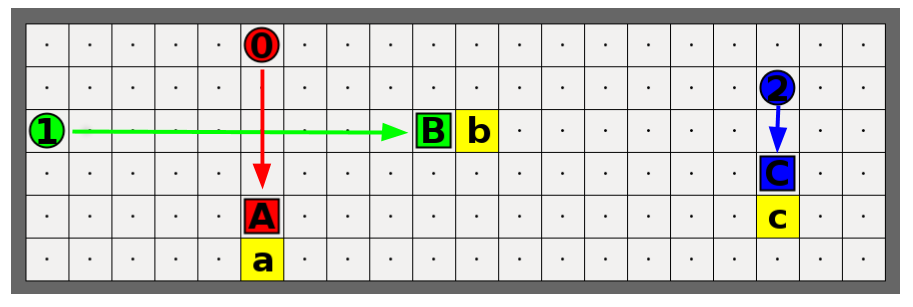
\includegraphics[width=0.8\textwidth]{figures/no_merge.png}
 \caption{Agent 2 does not need a plan merge}
 \label{fig:no_merge}
\end{center}
\end{figure}

\subsubsection{Plan merging conflict identification and solving}
\writer{Rafaela, Cosmin}

While merging plans, there are some situations where plan merging cannot possibly be made, even though all
possible plan intercalation options are tried. We have called this \textit{plan merging conflict}.

In order to make a good decision on how to solve such situations, we first need to identify them in a correct
way. In some situations, they can even be identified even before running the merging algorithm. One way in
which we have identified the apparition of a conflict is by analyzing if the paths of two agents are
colliding. Two paths collide if the end or the beginning of an agent’s path (that it has to follow in order to
complete a goal) is situated on another agent’s path and the two cannot avoid each other no matter how many
NoOp actions they might do while trying to merge their plans.

When a conflict is found\footnote{Either because the above mentioned method or simply because the plan merging
described in the section above fails}, agents need to solve it in order to be able to achieve their goals. The
conflict solving can be done by the central entity, it can be discussed between the conflicting agents or a
hybrid solution can be used. In our approach, we have considered the hybrid solution, in which the central
entity is the one identifying the conflicting situation, but then it contacts the agents so that they can come
up with possible solutions for solving the conflict. The steps of our plan conflict solving process can be
seen in Figure~\ref{fig:conflict_solving}. For the purpose of keeping simplicity, a situation with only 2
agents is presented.

\begin{figure}[htb]
\begin{center}
 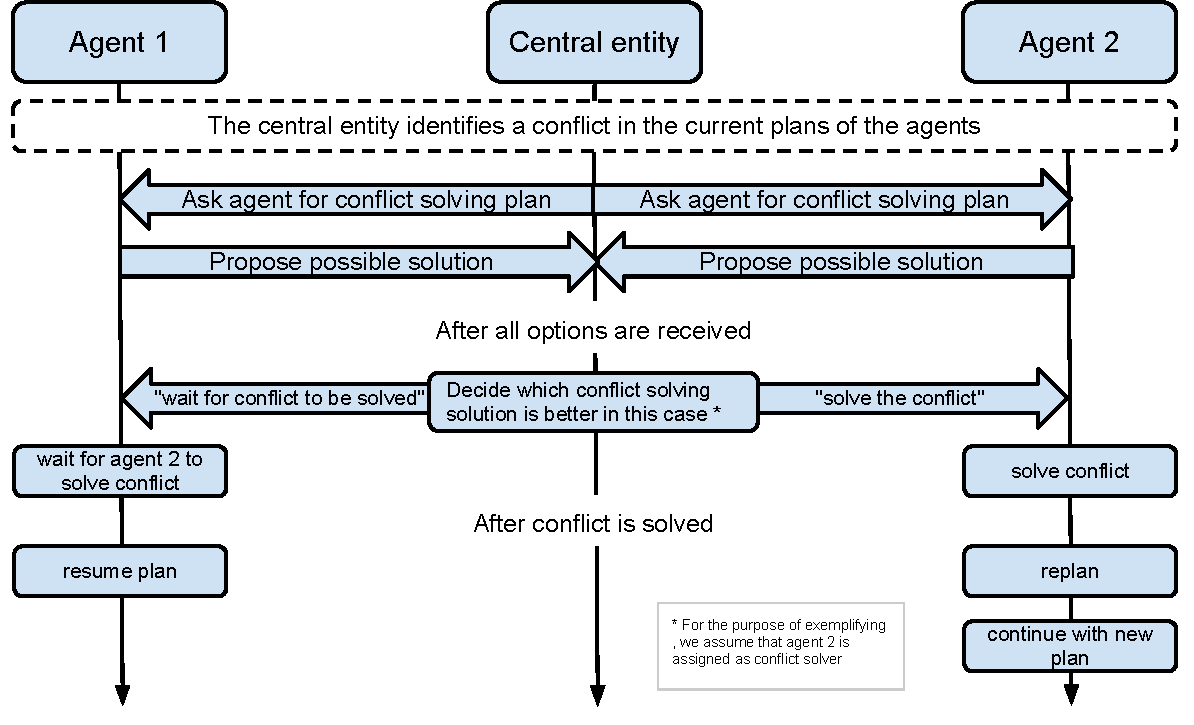
\includegraphics[width=0.7\textwidth]{figures/conflict_solving.pdf}
 \caption{Identifying and solving plan merging conflicts}
 \label{fig:conflict_solving}
\end{center}
\end{figure} 

Basically, the central entity will notice that there is a conflict based on the plans the agents submitted.
Identifying this, it will send a notification back to the agents asking them to propose a way to solve the
problem. Both agents compute their own solution for solving the conflict and send it back to the central
entity. The central entity can then decide, based on the costs of the solutions, which of the agents should
work on solving the conflict and which will need to wait for the other to finish its conflict solving plan
before resuming its initial plan. In the given example, agent 1 will wait for agent 2 to solve the conflict
and then agent 1 can resume its original plan. Agent 2 now needs to re-plan and see if it resumes the initial
plan (if it’s the best option) or if it chooses another goal which will lead for it to have a new plan.

Similarly to the case presented in section \ref{sec:plan_merging}, when two agents are conflicting and there
are other agents who are not, there is no need to make the agents which are not in conflict wait for the
conflict to be solved before they can continue their plans. In the situation that the plan chosen to solve
the conflict affects the plans of other agents (which were not originally in the conflict), then plan merging
or conflict solving is tried for the new affected agents.

\subsubsection{Agent cooperation}
\writer{Cosmin}
There are cases when agents cannot solve some situations or some goals by themselves, thus cooperation between
agents is required. One such situation is presented in figure \ref{fig:cooperation}. As we can see, agent 0 is
not able to reach box A in order to deliver it unless box B is moved out of its path. For this, agent 0 first
detects that he cannot reach box A, then it identifies that box B should be moved out of the way. After this,
other agents are asked to clear the path and agent 1 comes up with a plan to move B out of the way and return
to its initial position. After this, the central entity merges the plans of the 2 agents and the solution is
found.

\begin{figure}[htb]
\begin{center}
 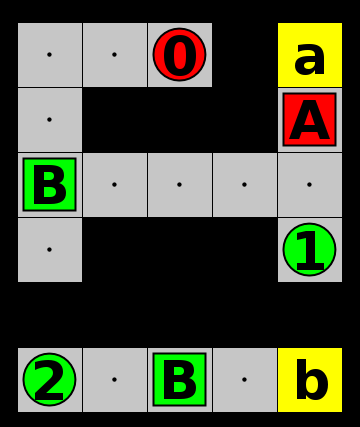
\includegraphics[width=0.35\textwidth]{figures/cooperation.png}
 \caption{Situation where agent cooperation is needed}
 \label{fig:cooperation}
\end{center}
\end{figure}

Thus, as identified from the situation above, the first thing that needs to be done is to identify when an
agent cannot fulfil its goal (in our example, agent 0 cannot reach box A). For this, we are first performing a
normal exploration looking for a solution. If no solution is found, we perform a second search starting with a
‘virtual’ state where boxes that cannot be moved by the agent are removed. If there is any way for the agent
to reach its goal, it will be identified in this second search and the boxes that block the path are
identified.

The second aspect needed to resolve scenarios such as the one presented above is how other agents are asked
for cooperation. In our system this was tackled based on the existing goals assigning/resolving
infrastructure. When an agent needs a path cleared, it communicates with the central entity which, in turn,
introduces a special type of Top Level Goal into the system. This is then handled like every other
goal\footnote{As mentioned in section \ref{sec:architecture}}: agents make estimations for the cost of solving
it, one of the agents gets assigned to work on it and then comes up with a plan. In the scenario above, only
agent 1 will come up with a goal solving cost estimation (as agent 2 cannot even reach box B) and will get
assigned to solve it.

\subsubsection{Partial observability}
\writer{Cosmin}

Our implementation is handling partial observability by identifying when one of the actions that was sent to
the server fails. As, due to applicability checks done when expanding states and when merging plans, there is
no possibility that a joint action has failed because of incompatible actions\footnote{E.g. an agent moving a
box in the same cell where there is another agent or another box}, cells which have unknown objects on them
are easily identified. Whenever this happens, our Central Entity is updating the beliefs of all the agents by
marking the cell as occupied in a central synchronized map representation. Further on, all the agents whose
plans might be affected by the newly discovered occupied cell are notified in order to replan.

\subsubsection{Heuristics}
\writer{Javier, Marius}
\label{sec:heuristics}

As previously stated, the A-Star search we used is guided by various heuristics, depending on what the current
subgoal is. Different heuristics were designed for having an agent get near a box or for having him move that
box.

For both types of goals, the heuristic takes into account the following: distance from the current cell to the
cell of the box, if the agent pushes or pulls another box, if the agent leaves boxes in cells with high
betweenness centrality, if the agent leaves boxes in other goal cells, if the agent blocks the access to other
goal cells, if the agent undoes a satisfied goal or if the agent pushes or pulls in a dead-end corridor.

A score is given for each of the measures and conditions mentioned above. These scores are multiplied by a
coefficient and added, resulting in the final heuristic score.

Depending on the type of the map, the values of the coefficient of each term is changed, thus resulting in
different heuristics for different types of maps.

For getting next to a box, the distance is the most important factor to be considered, as we usually want the
shortest path. However, if that shortest path is through another cell which has a satisfied goal, due to the
penalty for undoing goals, the computed path detours that cell, trying to find a better option according to
the cost of the path.

For moving the box to its goal cell, the agent is penalised, for example, for pulling in a dead-end corridor.
In Figure \ref{fig:heuristics1}, the agent needs to push box C to its goal, because if it pulls it, it would
be stuck in a dead-end and it would have to move box C from its goal, in order to be able to get out.

\begin{figure}[htb]
\begin{center}
 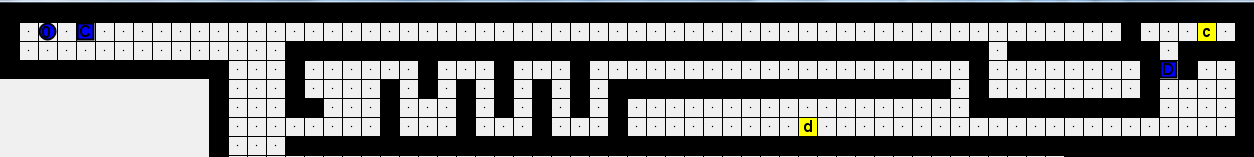
\includegraphics[width=0.8\textwidth]{figures/heuristics1.png}
 \caption{In this case, agent 0 needs to push box C to the goal, not pull it.}
 \label{fig:heuristics1}
\end{center}
\end{figure}

%something about hanoi? Javier? :D %

In some situations it is impossible to reach the box that the agent wants to deliver because there are some
other boxes blocking its path. In this situations it is necessary to clear the path for the agent. Figure
\ref{fig:heuristics2} shows a hanoi-like map, where the agent wants to deliver box A but the path is blocked
by other boxes and there is also a dead-end corridor.

For clearing the path the agent uses the dead-end corridors for storing the boxes that are in the middle of
its path. The final cell of each box is determined by the deepness of the dead-end. This means that the box is
pushed in the same direction while the betweenness centrality of a neighbour cell is lower than their own.

Another fact that it is necessary to take into account is that the first cell of the corridor must be empty,
in case that the agent needs this cell to make some turn movement, if it needs to change from pulling to
pushing.

\begin{figure}[htb]
\begin{center}
 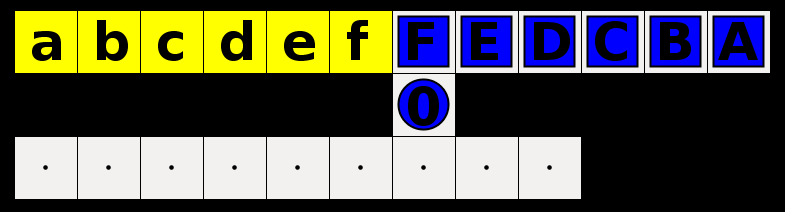
\includegraphics[width=0.6\textwidth]{figures/heuristics2.png}
 \caption{Hanoi-like map}
 \label{fig:heuristics2}
\end{center}
\end{figure}

\section{Results and findings}
\label{sec:results}
\writer{Alber, Javier, Marius, Ruxandra}

As the previous chapter has shown, our implementation is very complex and a variety of situations have been
taken into account. Due to our multi-agent, conflict solving and heuristics-based approach, as expected, the
program works very well on some types of maps,  but there are, of course, cases where it doesn't perform that
well. The most relevant cases will be analyzed further on.

\subsection{Single Agent}

The first thing we will analyse is how the system performs in a single-agent, deterministic environment.
Because of the heuristics we use, the solutions we are finding are near-optimal. Even though this is very good
for small maps, as the agent performs a really small number of actions, on large maps with a big number of
boxes, it takes a long time to compute the solution. However, due to the low-level optimizations done in our
implementation code, the search and expansions are extremely fast.

Another case in which the solution is very difficult to find is when there is a large number of boxes that
have to be moved out of the way for the agent to achieve its goal. This happens because the agent does not
know at the beginning how to move the boxes in a free space as it only has goals related to delivering a box
to a goal cell or clearing a path. In the future, a possible solution that we could use to solve this issue is
to add another type of goal for partially cleaning important and tricky parts of the map, which could be
assigned to each agent at the beginning.

Regarding the evaluation of the how the agents are being assigned the \textit{correct} goal, we have observed
that the defined heuristic was correctly guiding the agent to the optimal solution in all of our tests.

Figure~\ref{fig:goalplanneraresults}, presents an example of a solution produced by the system. Blue cells indicate boxes, while yellow cells indicate goal cells. Numbers indicate the order in which they were solved. It can be observed that the agent correctly identified the non-blocking goals as well as the ones that were closer to them (this is, the distance to the box, and from the box to the goal).

\begin{figure}[htb]

\begin{center}

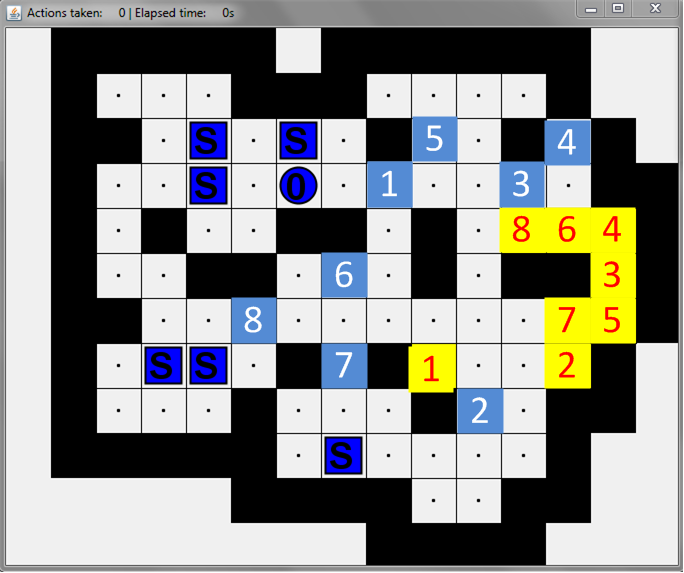
\includegraphics[width=0.4\textwidth]{figures/example_goal_planner}

\caption{Evaluation of the Goal Planner Heuristic}

\label{fig:goalplanneraresults}

\end{center}

\end{figure}

A side-effect of trying to find optimal solutions is that more time is needed in order to come up with the
solution. This is not very noticeable on small maps, but on larger maps, with more boxes, the time difference
can be easily observed.

After testing on various levels, we can say that the presented solution solves most of the Hanoi-like maps.
This is done with the special heuristic described in Section~\ref{sec:heuristics}..

Figure ~\ref{fig:results_hanoi} presents how the agent 0 is solving the map mentioned above, Figure
\ref{fig:heuristics2}.

\begin{figure}[htb]
\begin{center}
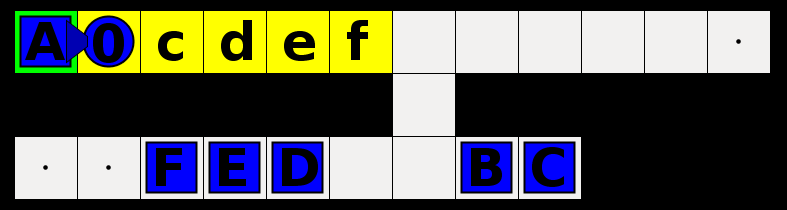
\includegraphics[width=0.5\textwidth]{figures/results_hanoi.png}
\caption{Agent 0 solving of the map in Figure \ref{fig:heuristics2}}
\label{fig:results_hanoi}
\end{center}
\end{figure}

An important aspect that should be mentioned when talking about heuristics is the pre-analysis of the map.
Because we can’t perform a complete analysis of the state at each step of the expansion as it would have been
very computationally demanding, we try to base our heuristic on information that can be computed before
starting the actual processing.

\subsection{Multi-agent} %FOMA / POMA
An observation which needs to be made is that the approach chosen was pure multi-agent planning, so each agent
creates its own plan, and only needs special communication with the central entity when conflicts are
detected. In some of the maps, multibody planning could have worked better. However, at least in theory,
multibody planning would not scale very well for large maps and a big number of agents. On the other hand, our
solution also had some problems with scaling for a large number of boxes/goals as the used heuristics did not
take all the parameters into account.

The result of multi-agent system in complex levels is not very good, because the central entity makes real
merging for each agent's plan, instead of just delaying one of the agents that are in conflict. While merging
works well when there is a conflict between only two agents as it finds the optimal merging in a reasonable
amount of time, it fails to work in cases where there are more than two agents and their actions can’t be
merged only by delaying and there is a need for extra-actions to be performed. Even though this solution is
time-consuming, it provides a solution that is more similar to a real-case scenario.

In POMA levels, the agents are capable of detecting the unknown objects that block their path and can recover
from this situation without any problems. Figure ~\ref{fig:poma_step1} shows how the agent wants to complete
its goal but finds an unknown object that stops it. Once the agent has updated its beliefs, it generates
another plan and tries again to complete its goal. Figure \ref{fig:poma_step2} presents how after some
interactions the agent manages to find the correct path.

\begin{figure}[htb]

\begin{center}

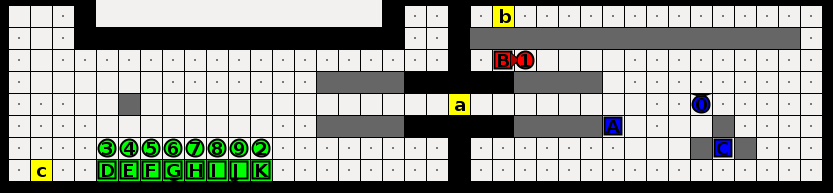
\includegraphics[width=0.8\textwidth]{figures/POMA_step1}

\caption{The agent 1 finds an unknown object in its path.}

\label{fig:poma_step1}

\end{center}

\end{figure}

\begin{figure}[htb]

\begin{center}

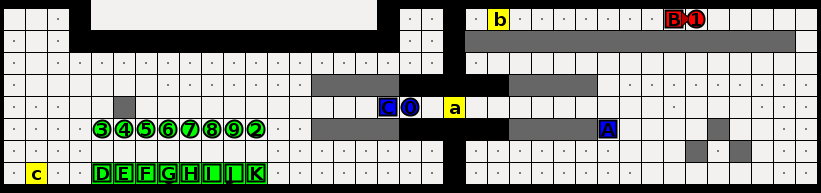
\includegraphics[width=0.8\textwidth]{figures/POMA_step2}

\caption{Agent 1 finally success in finding a path without unknown objects.}

\label{fig:poma_step2}

\end{center}

\end{figure}

The presented system has been tested in a competition against the projects developed by other students. The results show that the system is able to handle single agent maps with good results, being the group resolving in fewest actions in three of the thirteen maps, and resolving other two maps.

However, multiagent environments did not present the same performance, and results were not as good as expected. While we were able to find more optimal solutions by merging plans of the agents and replanning if necessary, the fact that we opted for a multiagent system instead of multibody had a huge impact the performance.

\section{Conclusions}
We have implemented a multi-agent infrastructure using the beliefs-desires-intention model. The agents are
capable of planning by themselves and a central unit merges the plans of the different agents when possible,
otherwise agents request other agents to help them or recompute new plans if necessary.

The results have shown that the system can resolve all three types of maps: FOSA, FOMA and POMA. The
performance on the first is good, although some improvements might be necessary to resolve complex scenarios.

\section{Further work}
Our implementation of the system allows anyone interested to easily add new heuristics, goal types or other
types of algorithms. Thus, after careful analyses or new observations, the system can be easily tweaked to
take into consideration new situations.

The most important aspect that can be improved in the case of our implementation is the plan merging conflict
resolution. In situations where the plans of more than two agents generate conflicts during the merging
process, the current implementation still lacks a strong way of resolution so improvements can be made.

Other aspects that can always be improved in artificial intelligence and multi-agent systems are the way
heuristics are computed and goal picking. Moreover, more low-level optimizations can be done in the core part
of the implementation for faster computations and better access to resources.

% Your references go at the end of the main text, and before the
% figures.  For this document we've used BibTeX, the .bib file
% scibib.bib, and the .bst file Science.bst.  The package scicite.sty
% was included to format the reference numbers according to *Science*
% style.




\bibliographystyle{Science}
\nocite{*}
\bibliography{scibib}



\end{document}




















